%%%%%%%%%%%%%%%%%%%%%%%%%%%%%%%%%%%%%%%%%%%%%%%%%%%%%%%%%%%%%%%%%%% 
%                                                                 %
%                            CHAPTER                              %
%                                                                 %
%%%%%%%%%%%%%%%%%%%%%%%%%%%%%%%%%%%%%%%%%%%%%%%%%%%%%%%%%%%%%%%%%%% 
\chapter{Analyse van de gebruikte data}
We testen de aanval beschreven in Hoofdstuk~\ref{chap:inferentieaanval} op een
dataset met activiteiten van een aantal gebruikers, om zo de kwetsbaarheid van
gebruikers van fitnessplatformen te evalueren. Maar het is dan ook essentieel
dat een representatieve dataset wordt gebruikt. We onderzoeken eigenschappen en
mogelijke afwijkingen of onregelmatigheden opdat we een gefundeerde conclusie
kunnen vormen, die eventueel bepaalde eigenschappen van de aard van de data mee
in rekening brengt.

Aangezien deze thesis voor een stuk verder bouwt op het onderzoek
van~\citeauthor{Dhondt}, is het handig om verder te werken met deze
dataset~\cite{Dhondt}. Dit maakt een directe vergelijking mogelijk. Deze
dataset werd volledig gescraped door~\citeauthor{Dhondt} vanaf de officiële
\ac{API} (\textit{strava.com/stream/ID}) van het platform
Strava\footnote{\url{https://www.strava.com/}}. De scope van deze dataset is
een periode van één week, startend op 11 juli 2021 00:00 \ac{UTC}. De site werd
chronologisch afgelopen voor alle activiteiten beschikbaar op het platform, met
sprongen van 9000 activiteiten. Let wel dat door mogelijke vertragingen door
bijvoorbeeld het uploaden van een activiteit, de activiteiten niet exact
chronologisch kunnen worden opgehaald. Indien een activiteit privaat is, of
reeds verwijderd is, dan zal deze worden overgeslagen en de volgende worden
genomen. Voor elke gevonden activiteit beschouwen we daarna de gebruiker. Van
alle bekomen gebruikers worden dan de rest van de activiteiten afgehaald en
bijgehouden in één grote dataset. De gegevens werden ook geanonimiseerd
opgeslagen, zodat de gebruikers niet meer kunnen worden geïdentificeerd. De
dataset bevat dus geen namen of andere persoonlijke gegevens, enkel willekeurig
toegekende ID's.

Deze thesis experimenteert echter slechts met een subset van 131 users, waarvan
er 101 gebruikt worden voor analyses en conclusies, en 30 voor het testen van
de aanval. Let wel, de fractie van de dataset die wij ter beschikking kregen is
met 101 gebruikers wel relatief klein, wat een vertekend beeld kan geven over
de werkelijkheid.

\section{Karakteristieken van de gebruikte dataset}
Op Figuur~\ref{fig:geographic_spread} is de geografische spreiding van de
activiteiten gevisualiseerd aan de hand van een heatmap. Hierop is duidelijk te
zien dat de meeste activiteiten zich in Centraal-Europa bevinden. Daarnaast is
ook een duidelijke concentratie te zien in de Verenigde Staten. In mindere mate
zijn ook activiteiten in Australië en Zuid-Amerika. De dataset bevat dus een
relatief grote spreiding van activiteiten over de hele wereld, wat een goede
basis is voor het testen van de aanval.

Op Tabel~\ref{tab:stats_dataset} zijn enkele globale statistieken met
betrekking tot gebruikers en de bijhorende activiteiten van de dataset
weergegeven. Er valt op dat de dataset per gebruiker toch meestal een groot
aantal activiteiten ter beschikking zijn. De gemiddelde gebruiker bevat 411
activiteiten, de mediaan is 296. Volgens de inferentieaanval beschreven in
Hoofdstuk~\ref{chap:inferentieaanval} resulteert een gebruiker met meer
activiteiten over het algemeen in een aanval met een hogere kans op slagen. Op
Figuur~\ref{fig:cdf_amount_activities} is de \ac{CDF} plot\footnote{Een
    Cumulative Distribution Function (CDF) plot is een grafiek die de cumulatieve
    verdeling van de waarden van een continue variabele
    weergeeft~\cite{CursusSt38:online}. De x-as van de grafiek bevat de
    verschillende waarden die de continue variabele kan aannemen, terwijl de y-as
    de kans aangeeft dat de variabele een waarde kleiner dan of gelijk aan die op
    de x-as aanneemt. De curve van de CDF laat zien hoe waarschijnlijk het is dat
    een willekeurige waarde van de continue variabele kleiner is dan een bepaalde
    drempelwaarde.} te zien die het aantal activiteiten per gebruiker weergeeft.
Hierop worden voorgaande besluiten enkel maar bevestigd. Het plot duidt ook aan
dat meer dan 20\% van de gebruikers een aantal activiteiten heeft dat groter is
dan 100.

\begin{figure}[h]
    \centering
    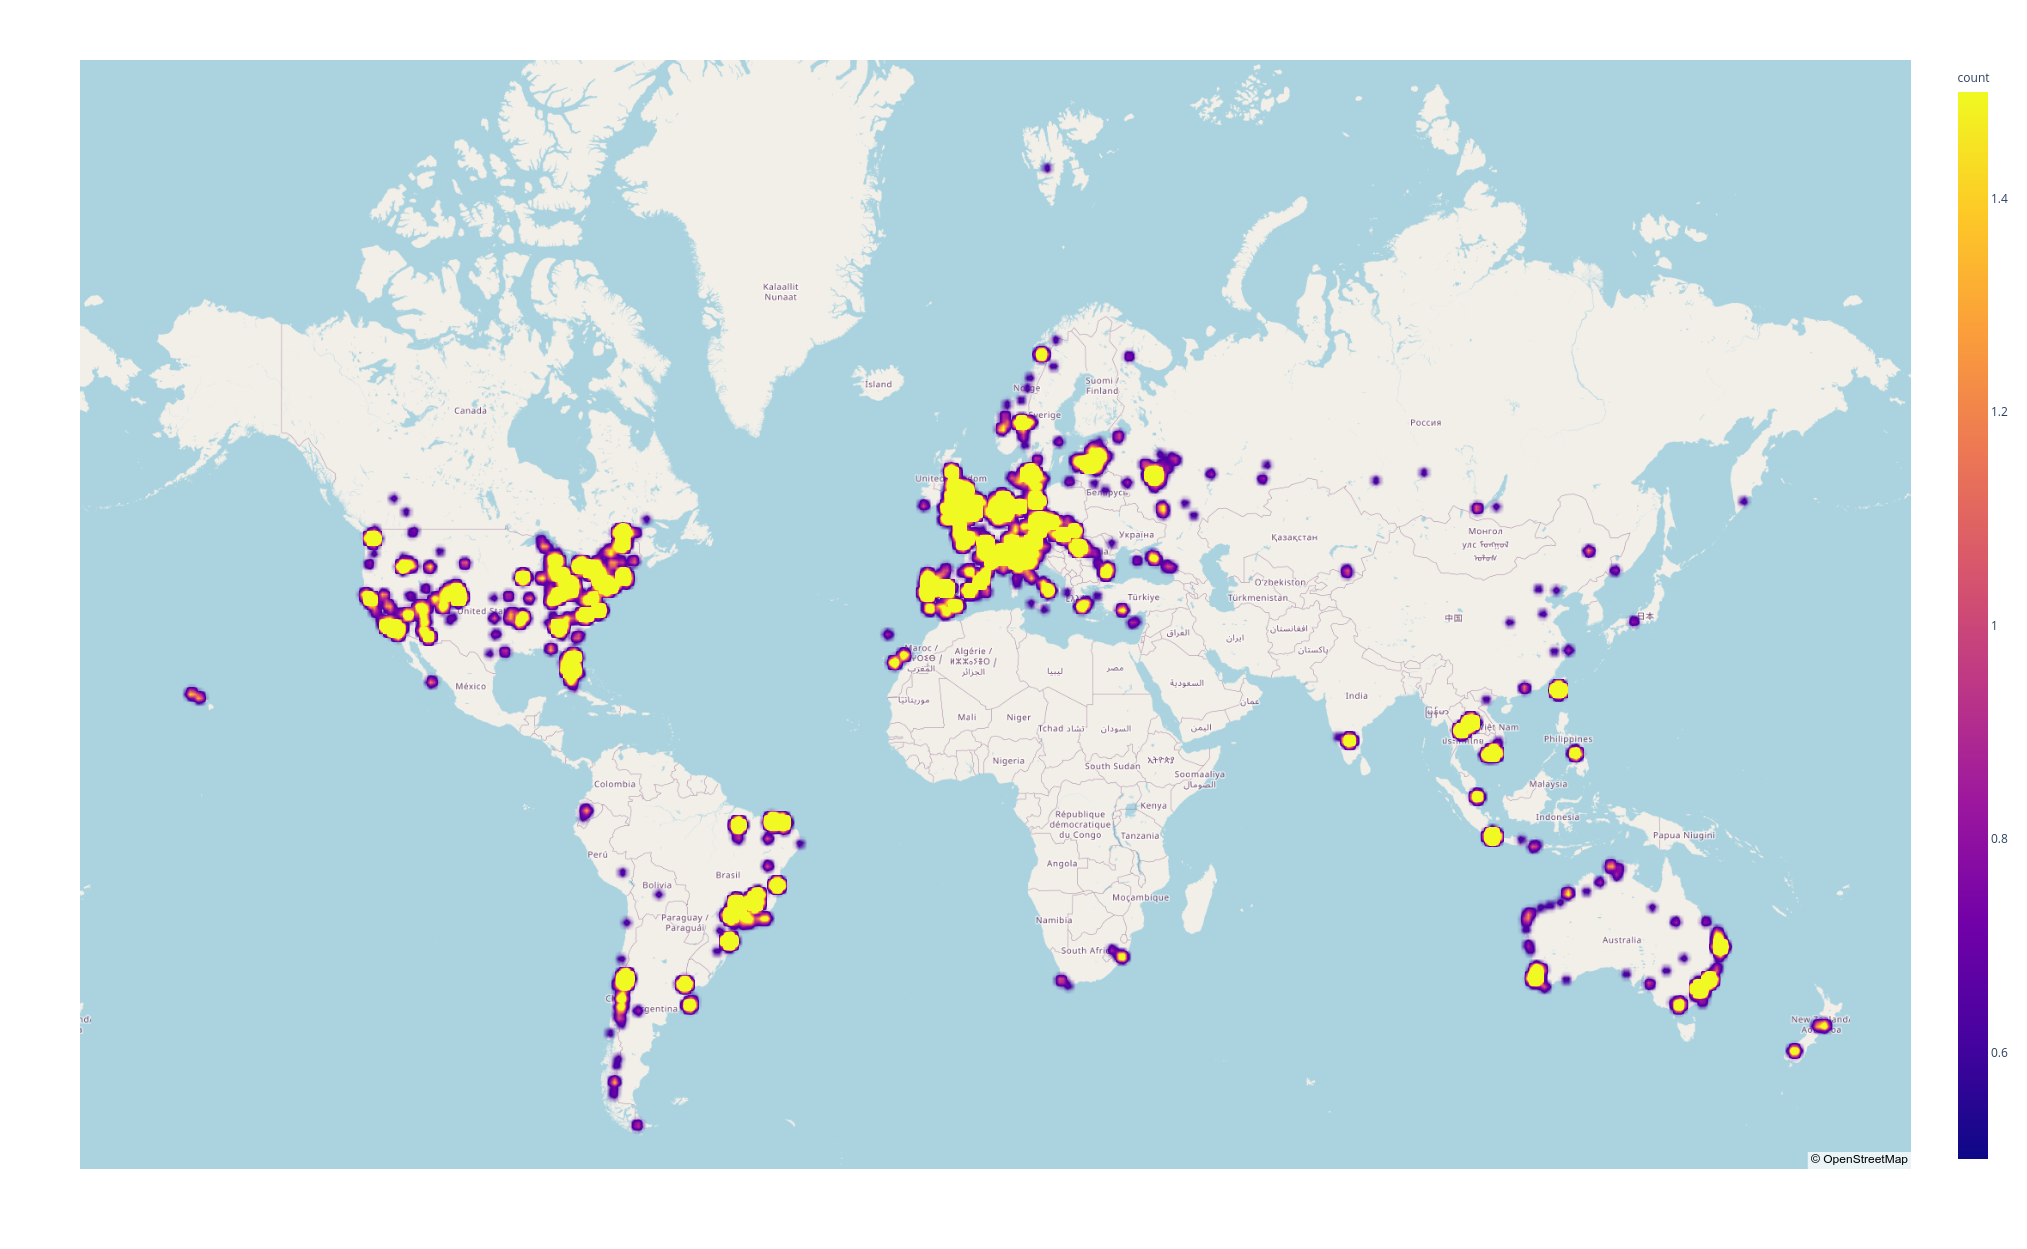
\includegraphics[width=\textwidth]{fig/Afwijkingen&Analyses/Heatmap.png}
    \caption{Geografische spreiding van de activiteiten in de dataset}\label{fig:geographic_spread}
\end{figure}
\begin{table}[h]
    \centering
    \begin{tabular}{|l||c|}
        \hline
                                                         & \textbf{Aantal} \\
        \hline \hline
        Totaal \# gebruikers                             & 101             \\
        \hline
        Totaal aantal activiteiten                       & 41 554          \\
        \hline
        Gemiddeld \# activiteiten per gebruiker          & 411             \\
        \hline
        Mediaan van het \# activiteiten per gebruiker    & 296             \\
        \hline
        Maximaal \# activities voor een enkele gebruiker & 2946            \\
        \hline
        Minimaal \# activities voor een enkele gebruiker & 31              \\
        \hline
    \end{tabular}
    \captionsetup{justification=centering}
    \caption{Overzicht van gebruikers en activiteiten}\label{tab:stats_dataset}
\end{table}
\begin{figure}[h]
    \centering
    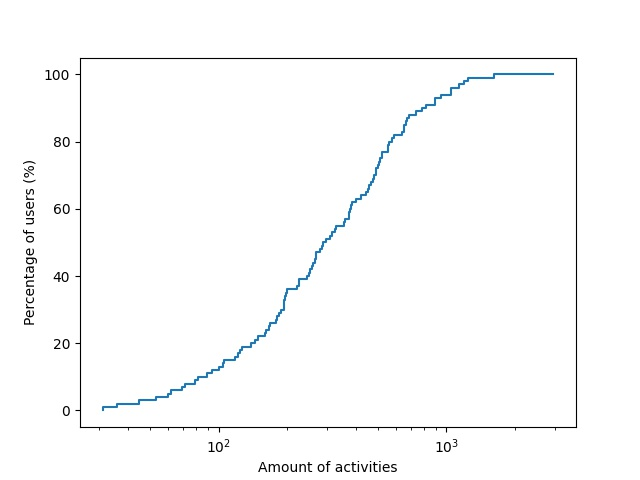
\includegraphics[width=0.9\textwidth]{fig/Afwijkingen&Analyses/CDF_amountActivities.jpg}
    \caption{CDF plot van het aantal activiteiten per gebruiker}\label{fig:cdf_amount_activities}
\end{figure}

% Let wel, alhoewel niet expliciet vermeld door~\citeauthor{Dhondt}, is er een
% vermoeden dat er bewust gezocht werd naar gebruikers met een zo groot mogelijk
% aantal activiteiten per gebruiker. Dit is een logische keuze, aangezien de
% aanval een hogere kans op slagen heeft bij users die meer activiteiten hebben.

% Let wel, de dataset is net een gemiddelde van 411 activiteiten per gebruiker
% niet volledig representatief voor de werkelijkheid. Wanneer we dit vergelijken
% met cijfers uit een studie die Strava zelf voerde in 2020, is er toch een
% mismatch terug te vinden~\cite{StravaMi72:online}. Het persbericht, waarvan
% Figuur~\ref{fig:3billionUsers} is overgenomen, stelt dat Strava in 2020 iets
% meer dan 50 miljoen gebruikers had, die samen in totaal drie miljard
% activiteiten op het platform hebben geplaatst. Indien we deze waarden omrekenen
% naar een gemiddelde, komen we uit op een ruwe geschatte 60 activiteiten per
% gebruiker ($\frac{3 \cdot 10^9}{5 \cdot 10^7} = 60 $). Dit is een stuk lager
% dan de gemiddelde 411 activiteiten per gebruiker in de dataset. De conclusies
% die dus getrokken worden uit deze steekproef mogen niet zomaar veralgemeend
% worden naar de volledige gebruikersbasis van Strava.
% \begin{figure}[h]
%     \centering
%     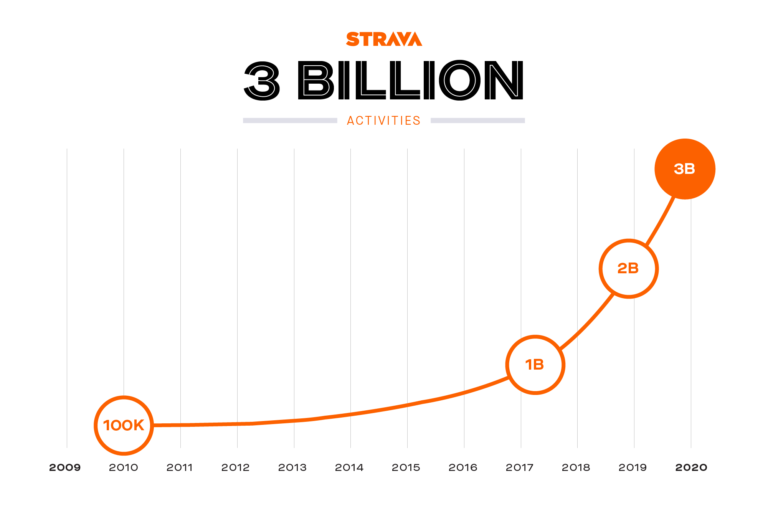
\includegraphics[width=0.7\textwidth]{fig/Strava_3billion.png}
%     \caption{Post op sociale media van Strava die de evolutie van het totaal aantal activiteiten weergeeft~\cite{StravaMi72:online}}\label{fig:3billionUsers}
% \end{figure}

% De oorzaak hiervan is mogelijks de manier waarop activiteiten worden afgehaald.
% Aangezien \citeauthor{Dhondt} met sprongen van 9000 een activiteit nemen, is de
% kans op terechtkomen bij een gebruiker die veel activiteiten heeft een stuk
% groter dan de kans dat terechtgekomen wordt op een gebruiker met een grote
% aantal activiteiten dan een gebruiker die wat minder actief is op het platform.

\section{Mogelijke afwijkingen binnenin de dataset}
Doordat de dataset niet expliciet werd gecheckt op onnauwkeurigheden en een
willekeurige sample is, is er een grote kans op activiteiten die afwijkingen of
fouten vertonen. Zeker door het belang van \ac{gps}-data in deze studie, die
een grote kans heeft op fouten, is het belangrijk om de dataset te analyseren
op mogelijke afwijkingen. Gps-data is een signaal die a.d.h.v.\ gekende
locaties van satellieten, gecombineerd met de tijd die het signaal nodig heeft
om vanaf de satelliet het toestel te bereiken, de locatie van een gebruiker kan
bepalen~\cite{BadGPSDa19:online}. Door de hoge snelheid van het signaal, kunnen
kleine vertragingen in het signaal al een grote invloed hebben op de
accuraatheid van de data. Andere factoren zoals hoge bomen of gebouwen, maar
ook de aanwezigheid van wolken kunnen een impact hebben op het signaal. Ook de
het interval waartussen opeenvolgende locaties worden bepaald, wat afhankelijk
is van het gebruikte toestel, kan meespellen. De soorten \ac{gps}-fouten die
kunnen optreden zijn reeds besproken in Sectie~\ref{sec:gps-fouten}.

Allereerst bestuderen we de aanwezigheid van \ac{gps}-fouten in de vorm van
signal losses of pauzes. Dit gebeurt door de afstand tussen twee opeenvolgende
\ac{gps}-punten te bestuderen.
Tabel~\ref{tab:distance_between_gps_points_table} geeft een globaal overzicht
van deze verdeling, en de volledige verdeling is terug te vinden op
Figuur~\ref{fig:distance_between_gps_points_CDF}. De gemiddelde afstand tussen
twee opeenvolgende locaties is $6.41$ meter, met een standaardafwijking van
$42.53$ meter. Het gemiddelde is relatief laag, wat kan wijzen op accurate
gegevens, maar de hoge standaardafwijking wijst op grote schommelingen. Op de
grafiek en in de tabel is te zien dat de meeste afstanden onder de $20$ meter
liggen, wat opnieuw een indicatie kan zijn van een degelijke precisie. Er is
echter wel een klein deel van de \ac{gps}-punten die een grote onderlinge
afstanden vertoond. Door de omvang van het aantal \ac{gps}-punten, en een
gemiddeld aantal punten per activiteit van $2574.90$, valt dit zeker niet te
verwaarlozen. Als we empirisch stellen dat een significant verschil $150$ meter
bedraagt, wat ongeveer drie maal de standaardafwijking voorsteld, dan ligt
0.2\% van de data boven deze drempel. Per activiteit zou dit dan resulteren op
gemiddeld $5.1$ afwijkende punten, wat zeker al kan zorgen voor een
significante afwijking op de resulterende afstand.
\begin{table}[h]
    \centering
    \begin{tabular}{lr}
        \toprule
        \midrule
        Total number of gps-points                    & $1.070 \cdot 10^8$       \\
        \hline
        distance between 2 gps points 20m $>$ 10m     & $13.91\%$                \\
        distance between 2 gps points 75m $>$ 50m     & $8.80 \cdot 10^{-1}\%$   \\
        distance between 2 gps points 100m $>$ 75m    & $9.11 \cdot 10^{-3}\%$   \\
        distance between 2 gps points 150m $>$ 100m   & $4.99 \cdot 10^{-3}\%$   \\
        distance between 2 gps points 200m $>$ 150m   & $1.97 \cdot 10^{-3}\%$   \\
        distance between 2 gps points 500m $>$ 200m   & $3.47 \cdot  10^{-3} \%$ \\
        distance between 2 gps points 1000m $>$ 500m  & $1.26 \cdot 10^{-3} \%$  \\
        distance between 2 gps points 2000m $>$ 1000m & $9.39 \cdot 10^{-4}$ \%  \\
        distance between 2 gps points $>$ 2000m       & $4.056 \cdot 10^{-4} \%$ \\
        \midrule
        \bottomrule
    \end{tabular}
    \captionsetup{justification=centering}
    \caption{Verdeling van de afstanden tussen twee opeenvolgende gps-punten}\label{tab:distance_between_gps_points_table}
\end{table}
\begin{figure}[h]
    \centering
    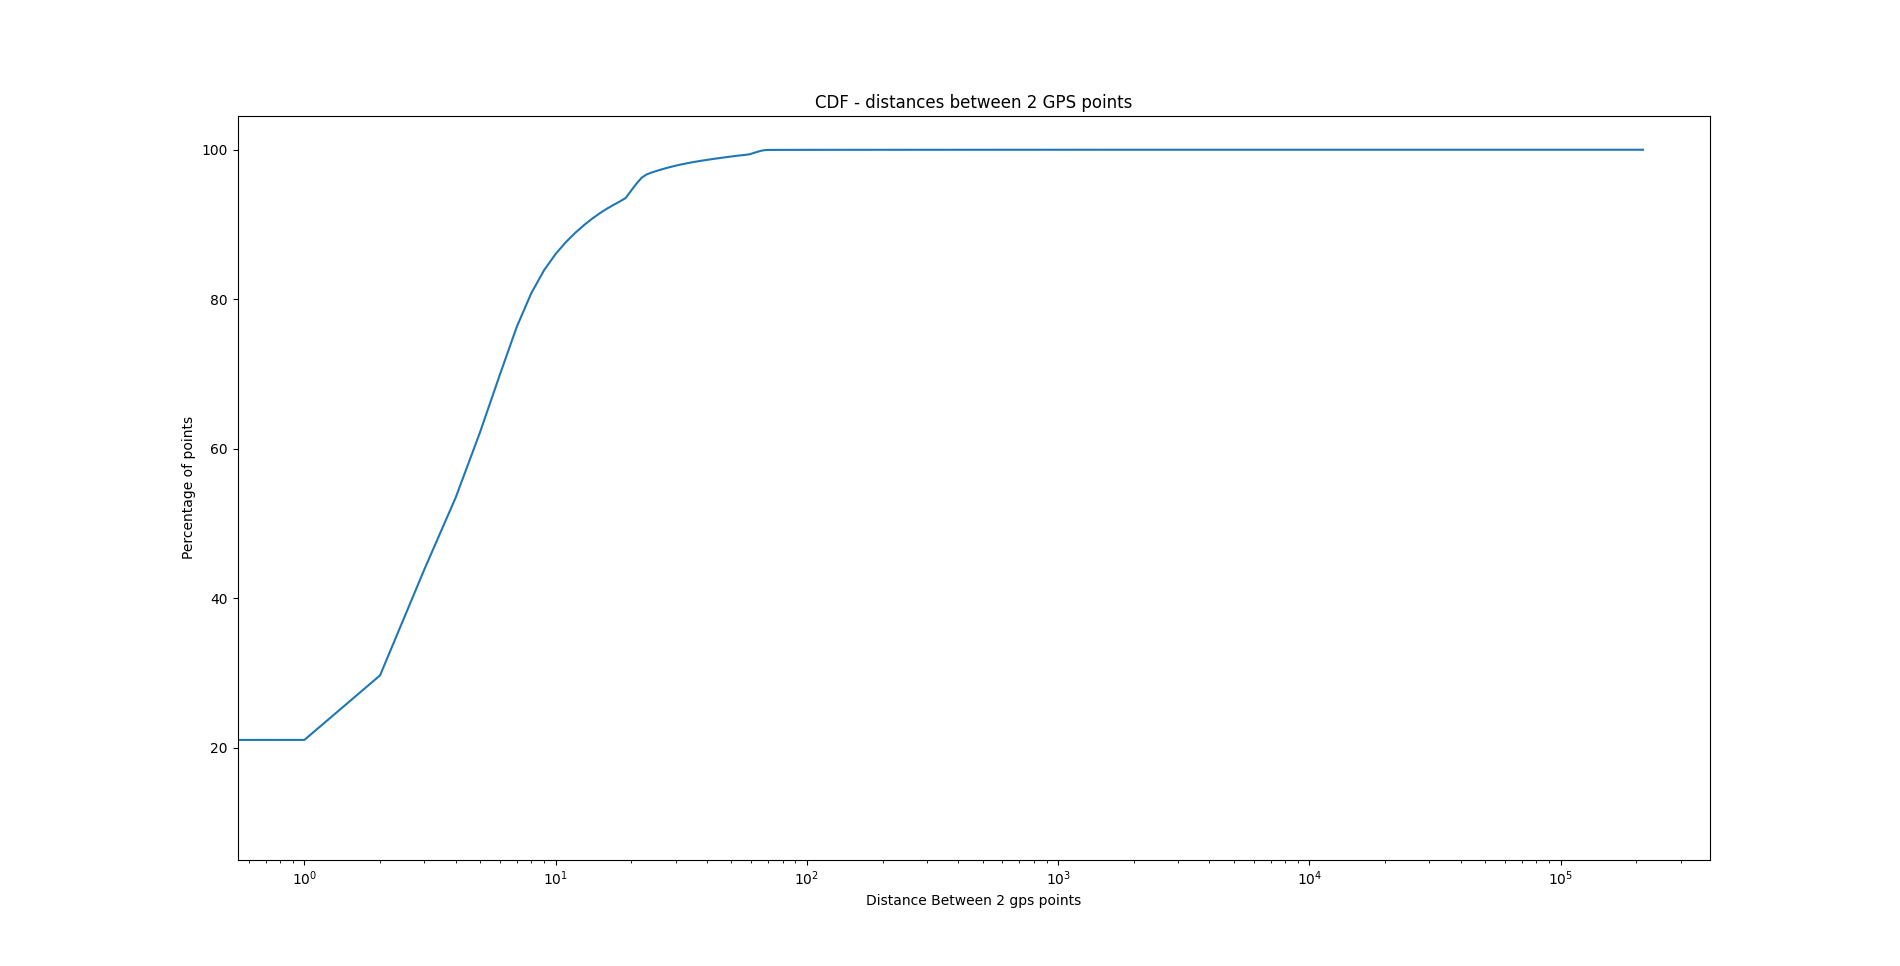
\includegraphics[width=\textwidth]{fig/Afwijkingen&Analyses/Graphs/Afstand tussen 2 gps-punten.png}
    \caption{Verdeling van de afstanden tussen twee opeenvolgende gps-punten}\label{fig:distance_between_gps_points_CDF}
\end{figure}

Om het aantal \ac{gps}-afwijkingen in de dataset te bepalen, wordt ook het
verschil onderzocht tussen de berekende afstand afgelegd binnen de \ac{EPZ}
(het zichtbare traject afgetrokken van de totale afstand) en de theoretisch
afgelegde afstand binnen de \ac{EPZ}, die af te lezen valt uit de dataset via
de cumulatieve afstand\footnote{Er wordt gesproken van een theoretische waarde,
    maar deze is eigenlijk de berekende waarde volgens het platform. We beschouwen
    deze dus als referentie.}. Een eerste visualisatie is te zien op
Figuur~\ref{fig:difference_noCDF}. De figuur illustreert de schommelingen
tussen de handmatig berekende afstand en de theoretische afstand van één
gebruiker. De pieken duiden op sterk afwijkende berekende afstanden, en dus ook
op grote \ac{gps}-fouten. Maar ook de schommelingen die iets minder opvallend
zijn duiden op grote inaccuraatheden tussen de berekende en theoretische
afstanden. De verschillen in de berekeningen voor de volledige dataset worden
weergegeven op Figuur~\ref{fig:differences_theoretical}. De figuur bevat de
\ac{CDF}-verdeling van de verschillen voor alle activiteiten, gebruik makend
van een logaritmische schaal. Op de grafiek valt op dat heel wat significante
verschillen aanwezig zijn. Dit duidt op het relatief zwaar doorwegen van de
\ac{gps}-fouten in de dataset. Aangezien het gaat over bepalen van woonplaatsen
of andere gevoelige locaties, kunnen afwijkingen vanaf 50 à 100 meter al sterk
doorwegen zijn. Daarnaast gaat het vaak over kleine afwijkingen op een heel wat
punten, wat kan resulteren in een grote afwijking. De grafieken tonen aan dat
er bij de ruwe ontvangen data heel wat \ac{gps}-fouten aanwezig zijn. Smoothing
zal dus zeker nodig zijn om deze te beperken.

\begin{figure}[h]
    \centering
    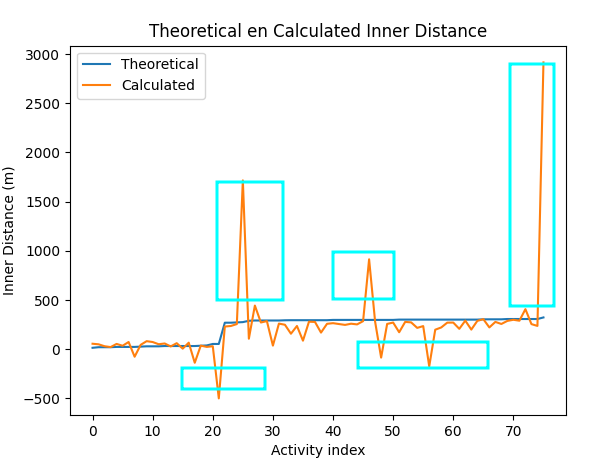
\includegraphics[width=0.7\textwidth]{fig/Afwijkingen&Analyses/Graphs/Verschil_Theoretische_innerDistance.png}
    \caption{Verschil tussen de berekende afstand en de theoretische afstand voor één gebruiker}\label{fig:difference_noCDF}
\end{figure}
\begin{figure}[h]
    \centering
    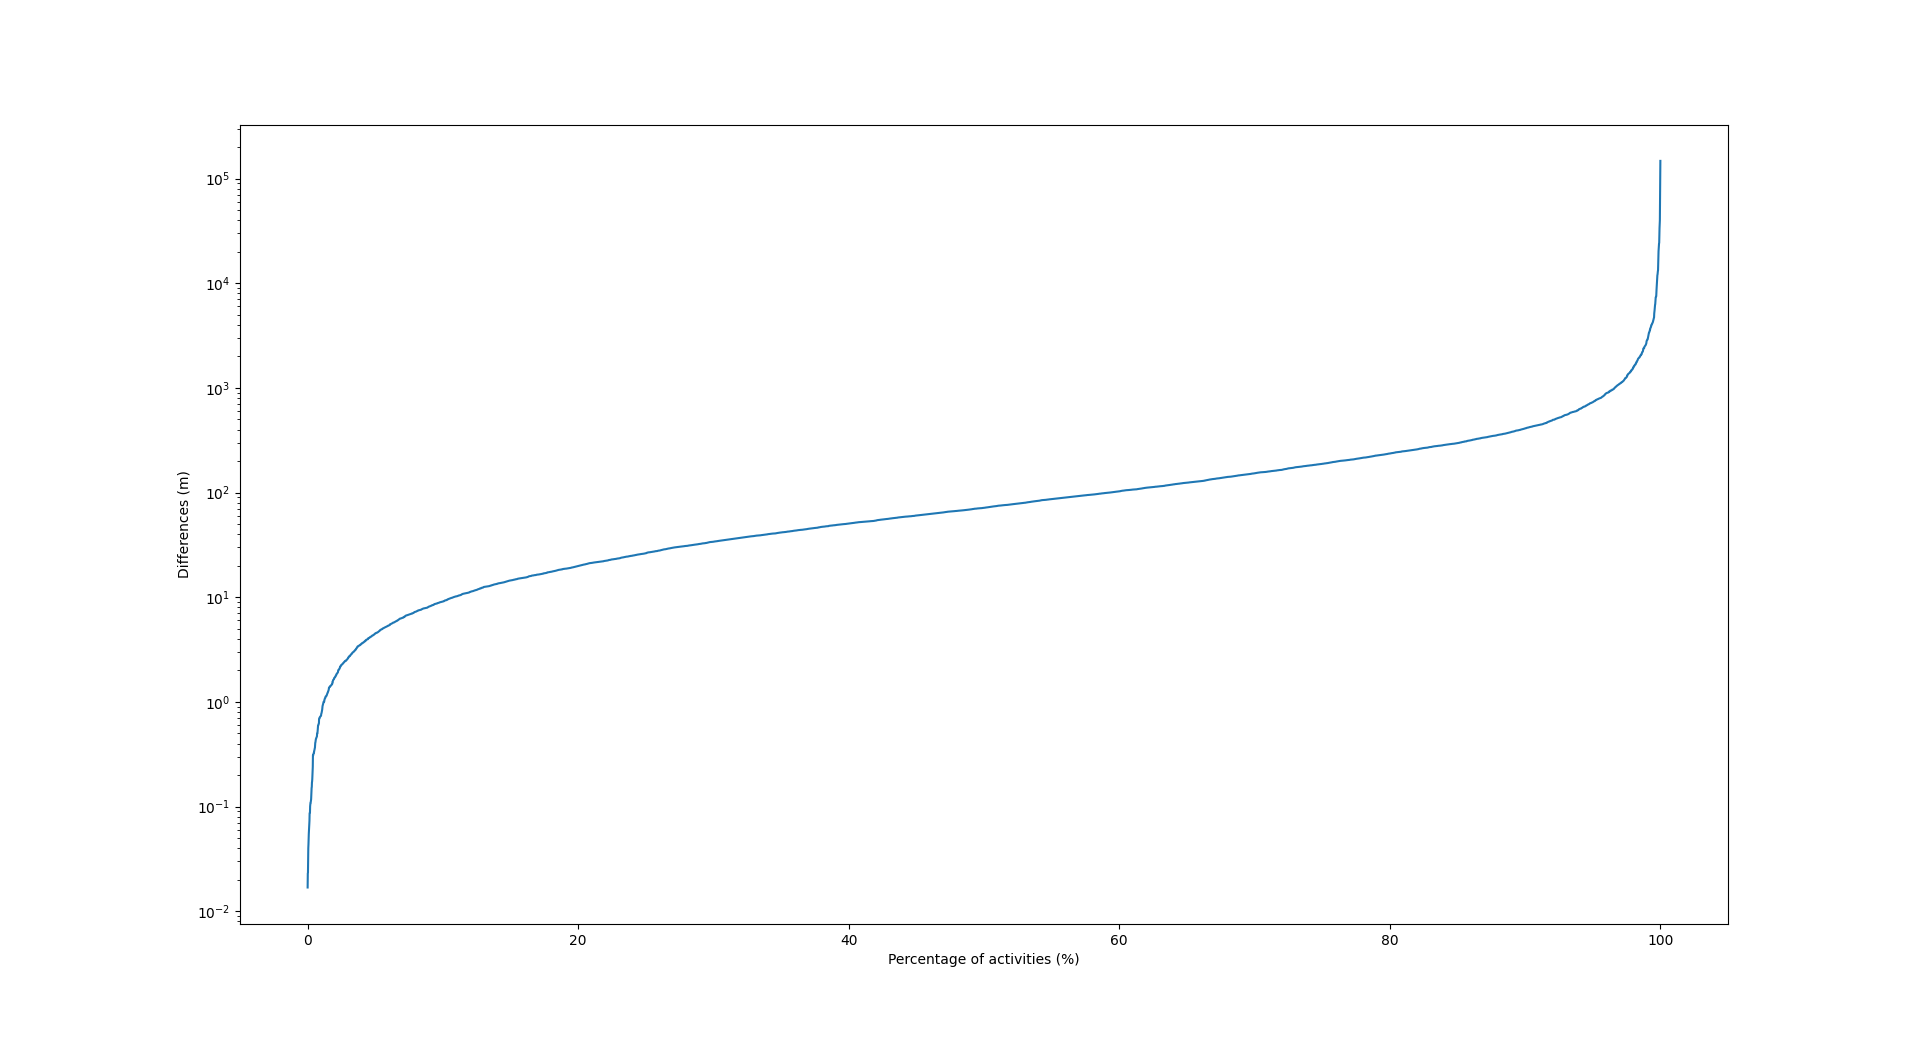
\includegraphics[width=\textwidth]{fig/Afwijkingen&Analyses/Graphs/100_Differences_tov_theoretische_BefSmoothening.png}
    \caption{Verdeling van het verschil tussen de berekende afstand en de theoretische afstand buiten de EPZ}\label{fig:differences_theoretical}
\end{figure}

\section{Technieken om gps-data te verbeteren}
Om de accuraatheid van de \ac{gps}-data te verbeteren, en zo een betere
\textit{outer distance} te kunnen berekenen en uiteindelijk een accuratere
aanval te bekomen, worden enkele technieken toegepast. Zoals besproken in
Sectie~\ref{sec:afstandsberekeningen_strava} is de hypothese dat de
fitnessplatformen ook gebruik maken van gelijkaardige technieken om de
\ac{gps}-data te verbeteren. De besproken technieken zijn \textit{map matching}
en \textit{\ac{gps}-smoothing}. Bij de uitvoering van de aanvallen wordt
smoothing toegepast. Er wordt dan ook geëxperimenteerd met verschillende
smoothing windows, op zoek naar het window met het beste effect op de aanval.

Daarnaast passen we ook een extra filtering toe die rekening houdt met
\ac{gps}-sprongen. Het idee is te stellen dat wanneer \ac{gps}-sprongen
gebeuren, en er dus een te grote afstand tussen twee opeenvolgende punten is,
deze afstand niet te laten meetellen. Dit is echter niet vanzelfsprekend,
aangezien dit waarschijnlijk wel op een andere manier in rekening gebracht
wordt door de platformen, bijvoorbeeld door map matching. Stel dat wij een
sprong van 150 meter laten vallen, maar de platformen laten deze wel meetellen,
dan zullen we de afwijking op het eindresultaat enkel maar verhogen. De drempel
voor de filtering moet dus hoog genoeg zijn om deze voorvallen te vermijden. In
dit onderzoek kozen we voor een drempelwaarde van 200 meter.